% Options for packages loaded elsewhere
\PassOptionsToPackage{unicode}{hyperref}
\PassOptionsToPackage{hyphens}{url}
%
\documentclass[
  11pt,
]{article}
\usepackage{lmodern}
\usepackage{amssymb,amsmath}
\usepackage{ifxetex,ifluatex}
\ifnum 0\ifxetex 1\fi\ifluatex 1\fi=0 % if pdftex
  \usepackage[T1]{fontenc}
  \usepackage[utf8]{inputenc}
  \usepackage{textcomp} % provide euro and other symbols
\else % if luatex or xetex
  \usepackage{unicode-math}
  \defaultfontfeatures{Scale=MatchLowercase}
  \defaultfontfeatures[\rmfamily]{Ligatures=TeX,Scale=1}
\fi
% Use upquote if available, for straight quotes in verbatim environments
\IfFileExists{upquote.sty}{\usepackage{upquote}}{}
\IfFileExists{microtype.sty}{% use microtype if available
  \usepackage[]{microtype}
  \UseMicrotypeSet[protrusion]{basicmath} % disable protrusion for tt fonts
}{}
\makeatletter
\@ifundefined{KOMAClassName}{% if non-KOMA class
  \IfFileExists{parskip.sty}{%
    \usepackage{parskip}
  }{% else
    \setlength{\parindent}{0pt}
    \setlength{\parskip}{6pt plus 2pt minus 1pt}}
}{% if KOMA class
  \KOMAoptions{parskip=half}}
\makeatother
\usepackage{xcolor}
\IfFileExists{xurl.sty}{\usepackage{xurl}}{} % add URL line breaks if available
\IfFileExists{bookmark.sty}{\usepackage{bookmark}}{\usepackage{hyperref}}
\hypersetup{
  pdftitle={Measurement invariance},
  hidelinks,
  pdfcreator={LaTeX via pandoc}}
\urlstyle{same} % disable monospaced font for URLs
\usepackage[margin=1in]{geometry}
\usepackage{longtable,booktabs}
% Correct order of tables after \paragraph or \subparagraph
\usepackage{etoolbox}
\makeatletter
\patchcmd\longtable{\par}{\if@noskipsec\mbox{}\fi\par}{}{}
\makeatother
% Allow footnotes in longtable head/foot
\IfFileExists{footnotehyper.sty}{\usepackage{footnotehyper}}{\usepackage{footnote}}
\makesavenoteenv{longtable}
\usepackage{graphicx,grffile}
\makeatletter
\def\maxwidth{\ifdim\Gin@nat@width>\linewidth\linewidth\else\Gin@nat@width\fi}
\def\maxheight{\ifdim\Gin@nat@height>\textheight\textheight\else\Gin@nat@height\fi}
\makeatother
% Scale images if necessary, so that they will not overflow the page
% margins by default, and it is still possible to overwrite the defaults
% using explicit options in \includegraphics[width, height, ...]{}
\setkeys{Gin}{width=\maxwidth,height=\maxheight,keepaspectratio}
% Set default figure placement to htbp
\makeatletter
\def\fps@figure{htbp}
\makeatother
\setlength{\emergencystretch}{3em} % prevent overfull lines
\providecommand{\tightlist}{%
  \setlength{\itemsep}{0pt}\setlength{\parskip}{0pt}}
\setcounter{secnumdepth}{5}
\usepackage{float}
\usepackage[autostyle, english = american]{csquotes}
\setlength{\parindent}{4em}
\setlength{\parskip}{2em}
\usepackage{setspace}\doublespacing
\usepackage{booktabs}
\usepackage{longtable}
\usepackage{array}
\usepackage{multirow}
\usepackage{wrapfig}
\usepackage{float}
\usepackage{colortbl}
\usepackage{pdflscape}
\usepackage{tabu}
\usepackage{threeparttable}
\usepackage{threeparttablex}
\usepackage[normalem]{ulem}
\usepackage{makecell}
\usepackage{xcolor}

\title{Measurement invariance}
\usepackage{etoolbox}
\makeatletter
\providecommand{\subtitle}[1]{% add subtitle to \maketitle
  \apptocmd{\@title}{\par {\large #1 \par}}{}{}
}
\makeatother
\subtitle{Ben Stenhaug \& Ben Domingue\\
Stanford University}
\author{}
\date{\vspace{-2.5em}}

\begin{document}
\maketitle
\begin{abstract}
ABSTRACT TO DO
\end{abstract}

{
\setcounter{tocdepth}{2}
\tableofcontents
}
\clearpage

\hypertarget{introduction}{%
\section{Introduction}\label{introduction}}

Inspired by Camilli (\protect\hyperlink{ref-camilli1992conceptual}{1992}), we view differential item functioning (DIF) as bias against a group of students that manifests when an item response model with too few ability dimensions is imposed. From this perspective, the term \enquote{differential item functioning} is, perhaps, a misnomer as DIF is a property of the student, not the item. For example, Ackerman (\protect\hyperlink{ref-ackerman1992didactic}{1992}) describes a scenario in which a test intends to measure a student's math ability, but performance also depends on their verbal ability. In this case, math ability is the \enquote{target ability,} and verbal ability is the \enquote{nuisance ability.} Fitting a unidimensional item response model to this test results in students with low verbal ability receiving a score systematically lower than their true math ability; therein lies the DIF.

Contrarily, the usual setup of DIF simulation studies frames DIF as a property of the item. For example, Kopf, Zeileis, and Strobl (\protect\hyperlink{ref-kopf2015framework}{2015}) simulate students as belonging to either a reference or focal group. They fix the item difficulties for the reference group, \({b_j}^{\text{ref}}\), to values from a previous study. They set item difficulties for the focal group to \({b_j}^{\text{foc}} = {b_j}^{\text{ref}}\) for items without DIF and \({b_j}^{\text{foc}} = {b_j}^{\text{ref}} + 0.6\) for items with DIF, where 0.6 is the magnitude of DIF in logits. They simulate student ability \({\theta_i}^{\text{ref}} \sim N(0,1)\) for students in the reference group and \({\theta_i}^{\text{foc}} \sim N(-1,1)\) for students in the focal group and generate item responses according to the Rasch model. The Rasch model specifies that the probability of student \(i\) responding correctly to item \(j\) is
\begin{align}
    P(y_{ij} = 1 | \theta_i, b_j) = \sigma(\theta_i - b_j)
\end{align}
where \(\sigma(x) = \frac{e^x}{e^x + 1}\) is the standard logistic function.

We find it more informative to describe simulation conditions in terms of single-dimensional items and multidimensional abilities. For example, to translate the Kopf, Zeileis, and Strobl (\protect\hyperlink{ref-kopf2015framework}{2015}) simulation from the DIF-as-item-property view to the DIF-as-student-property view, item difficulty is set to what was previously \({b_j}^{\text{ref}}\) for all students. Student ability is expanded to two dimensions, the target ability dimension and nuisance ability dimension. The target ability is what was previously just ability where \({\theta_i}^{\text{ref}} \sim N(0,1)\) for students in the reference group and \({\theta_i}^{\text{foc}} \sim N(-1,1)\) for students in the focal group. The nuisance ability is set to \({\eta_i}^{\text{ref}} = 0\) for the reference group and \({\eta_i}^{\text{ref}} = -1\) for the focal group. We now need to use a 2PL model where the slope on target ability \(a_{1j} = 1\) for all items (consistent with the Rasch model) and the slope on nuisance ability \(a_{2j} = 0.6\) for all items with DIF and \(a_{2j} = 0\) otherwise. Again, 0.6 is the magnitude of DIF in logits. According to the two-dimensional 2PL model, the probability student \(i\) responding correctly to item \(j\) is
\begin{align}
    P(y_{ij} = 1 | \theta_i, \eta_i, a_{1j}, a_{2j}, b_j) = \sigma(a_{1j}\theta_i + a_{2j}\eta_i - b_j).
\end{align}
This translation between views makes explicit that nearly all DIF simulation studies have, perhaps suboptimally, examined the unrealistic scenario in which the variance of the nuisance ability is set to 0 for all students in the same group.

If we insist on describing simulation conditions from the DIF-as-student-property view, one might wonder the following: Why not fit a multidimensional item response model which describes the data fully instead of looking for bias in a lower-than-necessary dimensional model? Camilli (\protect\hyperlink{ref-camilli1992conceptual}{1992}, 144) tested this idea with the goal of a \enquote{more satisfying description of the secondary abilities.} He found that the rotational indeterminacy of item response models is challenging to overcome and concluded that \enquote{a priori knowledge of the true factor structure} is necessary. It's hard to imagine how one would have such knowledge. Therefore, the best approach, which the DIF literature has nearly unanimously taken, is to fit unidimensional item response models and then look for bias manifesting in the item parameters.

\hypertarget{dif-methods}{%
\section{DIF methods}\label{dif-methods}}

Psychometricians have long been in search of the perfect DIF detection method. Meade and Wright (\protect\hyperlink{ref-meade2012solving}{2012}) compared the most commonly used methods and unequivocally recommended the all-others-as-anchors (AOAA) method, where each item is tested one at a time for DIF using all other items as anchors. More specifically, testing is done using a nested model comparison between the baseline model, where all item parameters are fixed across groups, and the flexible model, where the parameters of the tested item are freed across groups. Anchor items have fixed parameters across groups and consequently are used to estimate the ability difference between groups. For example, Edelen et al. (\protect\hyperlink{ref-edelen2006identification}{2006}) used AOAA to look for DIF between the English and Spanish versions of the 21-item Mini-Mental State Examination and found that 10 of the 21 items exhibited DIF. How can we be sure its those 10 items and not the other 11 items with DIF? Implicit in the use of AOAA is the assumption that all items not being tested do not exhibit DIF, which is, of course, impossible. Undesirably, most applications of DIF methods and many simulation studies do not make explicit the assumptions of the DIF method Strobl et al. (\protect\hyperlink{ref-strobl2018anchor}{2018}). In this way, psychometricians might benefit from adopting economists' habit of explicitly stating assumptions and debating their plausibility.

Researchers have noticed the circular logic of AOAA, but have mostly described it indirectly by pointing out inflated Type I errors in simulation studies (Stark, Chernyshenko, and Drasgow \protect\hyperlink{ref-stark2006detecting}{2006}). A simple thought experiment illustrates how AOAA fails: Imagine a test with three items where the first item has DIF, and the other two do not. Using AOAA, all items test positive for DIF. The last two items incorrectly test positive because including the first item in the anchor set causes the group ability difference to be misestimated. This phenomenon of items with real DIF inducing the appearance of DIF in other items was only indirectly discussed in the literature until (Andrich and Hagquist \protect\hyperlink{ref-andrich2012real}{2012}) coined the term \enquote{artificial DIF.}

One way to attempt to counter artificial DIF is with purification with iterative anchor selection. For example, (Drasgow \protect\hyperlink{ref-drasgow1987study}{1987}) started with AOAA, removed items displaying DIF from the anchor set, then continued iteratively to test the remaining items for DIF until no more items tested positively. (Kopf, Zeileis, and Strobl \protect\hyperlink{ref-kopf2015framework}{2015}) named this technique Iterative-backward-AOAA with \enquote{backward} (as in reverse, not incorrect) referring to beginning with the assumption that all items are DIF free. Iterative-backward-AOAA might seem like an improvement, but what does one do when all items display DIF in the first AOAA stage? With a sufficient sample size, this will necessarily be the case. Kopf, Zeileis, and Strobl (\protect\hyperlink{ref-kopf2015framework}{2015}) encountered precisely this problem in their simulation study and chose to select a single anchor item randomly. Woods suggested a more straightforward, one-step method which uses AOAA and selects the, say, four items that exhibit the least amount of DIF. It's unclear if one should proceed if those four items display DIF themselves.

We propose an extension of these methods, all-others-as-anchors-one-at-a-time (AOAA-OAT), which, to our knowledge, has not previously been proposed. AOAA-OAT starts with AOAA, and the single item exhibiting the most DIF is removed from the anchor set. Each item in the anchor set is then tested for DIF again (with items outside of the anchor set allowed to have free parameters across groups in both the baseline and flexible model). This process continues until no new items display DIF. Applying AOAA-OAT to our thought experiment demonstrates its logic. The initial AOAA removes the real DIF item from the anchor set because it exhibits the most DIF. In the next step, both of the other items test negative for DIF, and we arrive at the correct conclusion. AOAA-OAT has two assumptions: First, that at least one item does not have DIF, and second, that the majority of items do not have DIF.

DIF methods, in general, seem to be designed to automatically detect items with DIF without any intervention from a human. In some cases, it might make sense to present information to the analyst in a way that empowers them to make decisions. Our preferred technique, which we refer to as the \enquote{equal means logit graph} (EMLG), is to set both groups means to 0 so that differences in performance to manifest in the item parameters. Relatedly, Pohl, Stets, and Carstensen (\protect\hyperlink{ref-pohl2017cluster}{2017}) fit a model with both groups means set to 0 in a pedagogical example, and Talbot III (\protect\hyperlink{ref-talbot2013taking}{2013}) fixed both pre-test and post-test means to 0 in order to estimate item-specific learning gains.

We use a simple simulation to demonstrate EMLG. 10,000 reference group students and 10,000 focal group students take an eight-item test. Target ability is simulated \({\theta_i}^{\text{ref}} \sim N(0,1)\) for students in the reference group and \({\theta_i}^{\text{foc}} \sim N(-1,1)\) for students in the focal group. Nuisance ability is set to \({\eta_i}^{\text{ref}} = 0\) for the reference group and \({\eta_i}^{\text{ref}} = -1\) for the focal group. The slope on target ability is set to \(a_{1j} = 1\) for all items, and the slope on nuisance ability is set to \(a_{2j} = 0.5\) for the last three items (the items with DIF) and \(a_{2j} = 0\) otherwise. We fit a unidimensional Rasch, with both group means fixed to 0, to the simulated item response data. We estimate the item parameter covariance matrix using Oakes' identity (Chalmers \protect\hyperlink{ref-chalmers2018numerical}{2018}). Multiple imputations (MI) (Yang, Hansen, and Cai \protect\hyperlink{ref-yang2012characterizing}{2012}) are used to estimate the distribution of the difference in difficulty, \({b_j}^{\text{foc}} - {b_j}^{\text{ref}}\), for each item. Figure \ref{fig:emlg} shows these distributions.

\begin{figure}[H]

{\centering 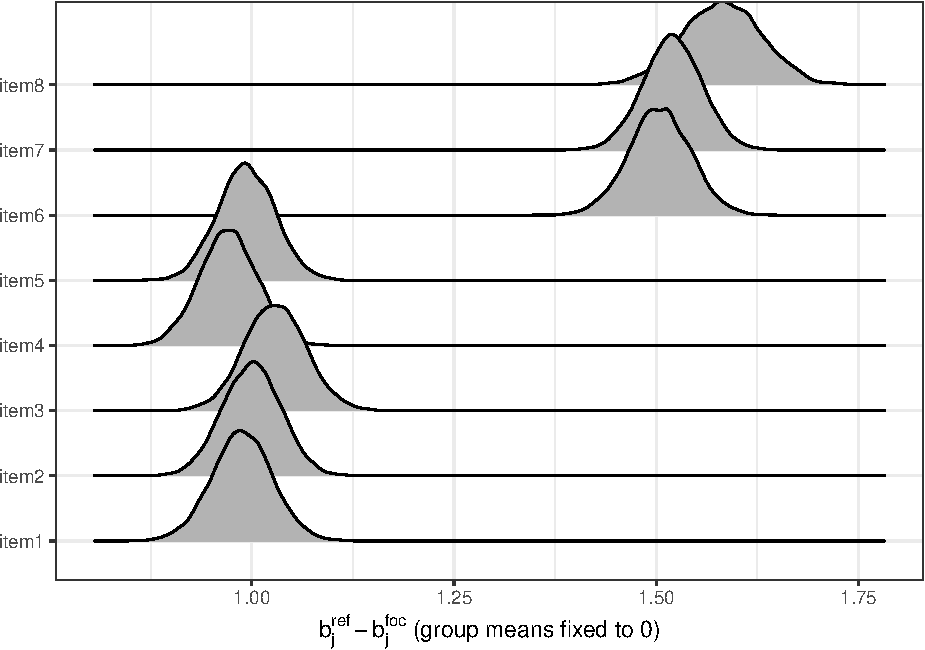
\includegraphics[width=0.7\linewidth]{paper_files/figure-latex/emlg-1} 

}

\caption{Equal means logit graph (EMLG)}\label{fig:emlg}
\end{figure}

\hypertarget{references}{%
\section{References}\label{references}}

\hypertarget{refs}{}
\leavevmode\hypertarget{ref-ackerman1992didactic}{}%
Ackerman, Terry A. 1992. ``A Didactic Explanation of Item Bias, Item Impact, and Item Validity from a Multidimensional Perspective.'' \emph{Journal of Educational Measurement} 29 (1): 67--91.

\leavevmode\hypertarget{ref-andrich2012real}{}%
Andrich, David, and Curt Hagquist. 2012. ``Real and Artificial Differential Item Functioning.'' \emph{Journal of Educational and Behavioral Statistics} 37 (3): 387--416.

\leavevmode\hypertarget{ref-camilli1992conceptual}{}%
Camilli, Gregory. 1992. ``A Conceptual Analysis of Differential Item Functioning in Terms of a Multidimensional Item Response Model.'' \emph{Applied Psychological Measurement} 16 (2): 129--47.

\leavevmode\hypertarget{ref-chalmers2018numerical}{}%
Chalmers, R Philip. 2018. ``Numerical Approximation of the Observed Information Matrix with Oakes' Identity.'' \emph{British Journal of Mathematical and Statistical Psychology} 71 (3): 415--36.

\leavevmode\hypertarget{ref-drasgow1987study}{}%
Drasgow, Fritz. 1987. ``Study of the Measurement Bias of Two Standardized Psychological Tests.'' \emph{Journal of Applied Psychology} 72 (1): 19.

\leavevmode\hypertarget{ref-edelen2006identification}{}%
Edelen, Maria Orlando, David Thissen, Jeanne A Teresi, Marjorie Kleinman, and Katja Ocepek-Welikson. 2006. ``Identification of Differential Item Functioning Using Item Response Theory and the Likelihood-Based Model Comparison Approach: Application to the Mini-Mental State Examination.'' \emph{Medical Care}, S134--S142.

\leavevmode\hypertarget{ref-kopf2015framework}{}%
Kopf, Julia, Achim Zeileis, and Carolin Strobl. 2015. ``A Framework for Anchor Methods and an Iterative Forward Approach for Dif Detection.'' \emph{Applied Psychological Measurement} 39 (2): 83--103.

\leavevmode\hypertarget{ref-meade2012solving}{}%
Meade, Adam W, and Natalie A Wright. 2012. ``Solving the Measurement Invariance Anchor Item Problem in Item Response Theory.'' \emph{Journal of Applied Psychology} 97 (5): 1016.

\leavevmode\hypertarget{ref-pohl2017cluster}{}%
Pohl, Steffi, Eric Stets, and Claus H Carstensen. 2017. ``CluStEr-baSEd anCHor Item Identification and Selection.'' NEPS Working Paper.

\leavevmode\hypertarget{ref-stark2006detecting}{}%
Stark, Stephen, Oleksandr S Chernyshenko, and Fritz Drasgow. 2006. ``Detecting Differential Item Functioning with Confirmatory Factor Analysis and Item Response Theory: Toward a Unified Strategy.'' \emph{Journal of Applied Psychology} 91 (6): 1292.

\leavevmode\hypertarget{ref-strobl2018anchor}{}%
Strobl, Carolin, Julia Kopf, Raphael Hartmann, and Achim Zeileis. 2018. ``Anchor Point Selection: An Approach for Anchoring Without Anchor Items.'' Working Papers in Economics; Statistics.

\leavevmode\hypertarget{ref-talbot2013taking}{}%
Talbot III, Robert M. 2013. ``Taking an Item-Level Approach to Measuring Change with the Force and Motion Conceptual Evaluation: An Application of Item Response Theory.'' \emph{School Science and Mathematics} 113 (7): 356--65.

\leavevmode\hypertarget{ref-yang2012characterizing}{}%
Yang, Ji Seung, Mark Hansen, and Li Cai. 2012. ``Characterizing Sources of Uncertainty in Item Response Theory Scale Scores.'' \emph{Educational and Psychological Measurement} 72 (2): 264--90.

\end{document}
